The Elevator is controlled by sending a hex encoded signal via serial cable.
In order to move the elevator to floor three, we are sending a signal which is interpreted as a move command to floor three.
We can also send a special "heartbeat" signal that will make the elevator respond with the information about the current floor it is on.
So, when the user enters the elevator cabin and asks to take him to certain floor, the user utterance is recognized and the corresponding floor signal is sent.
After the elevator receives the signal it should close the doors and start moving if everything went well.

% we need a few pics here when we finish the setup
%\begin{figure}
%\center{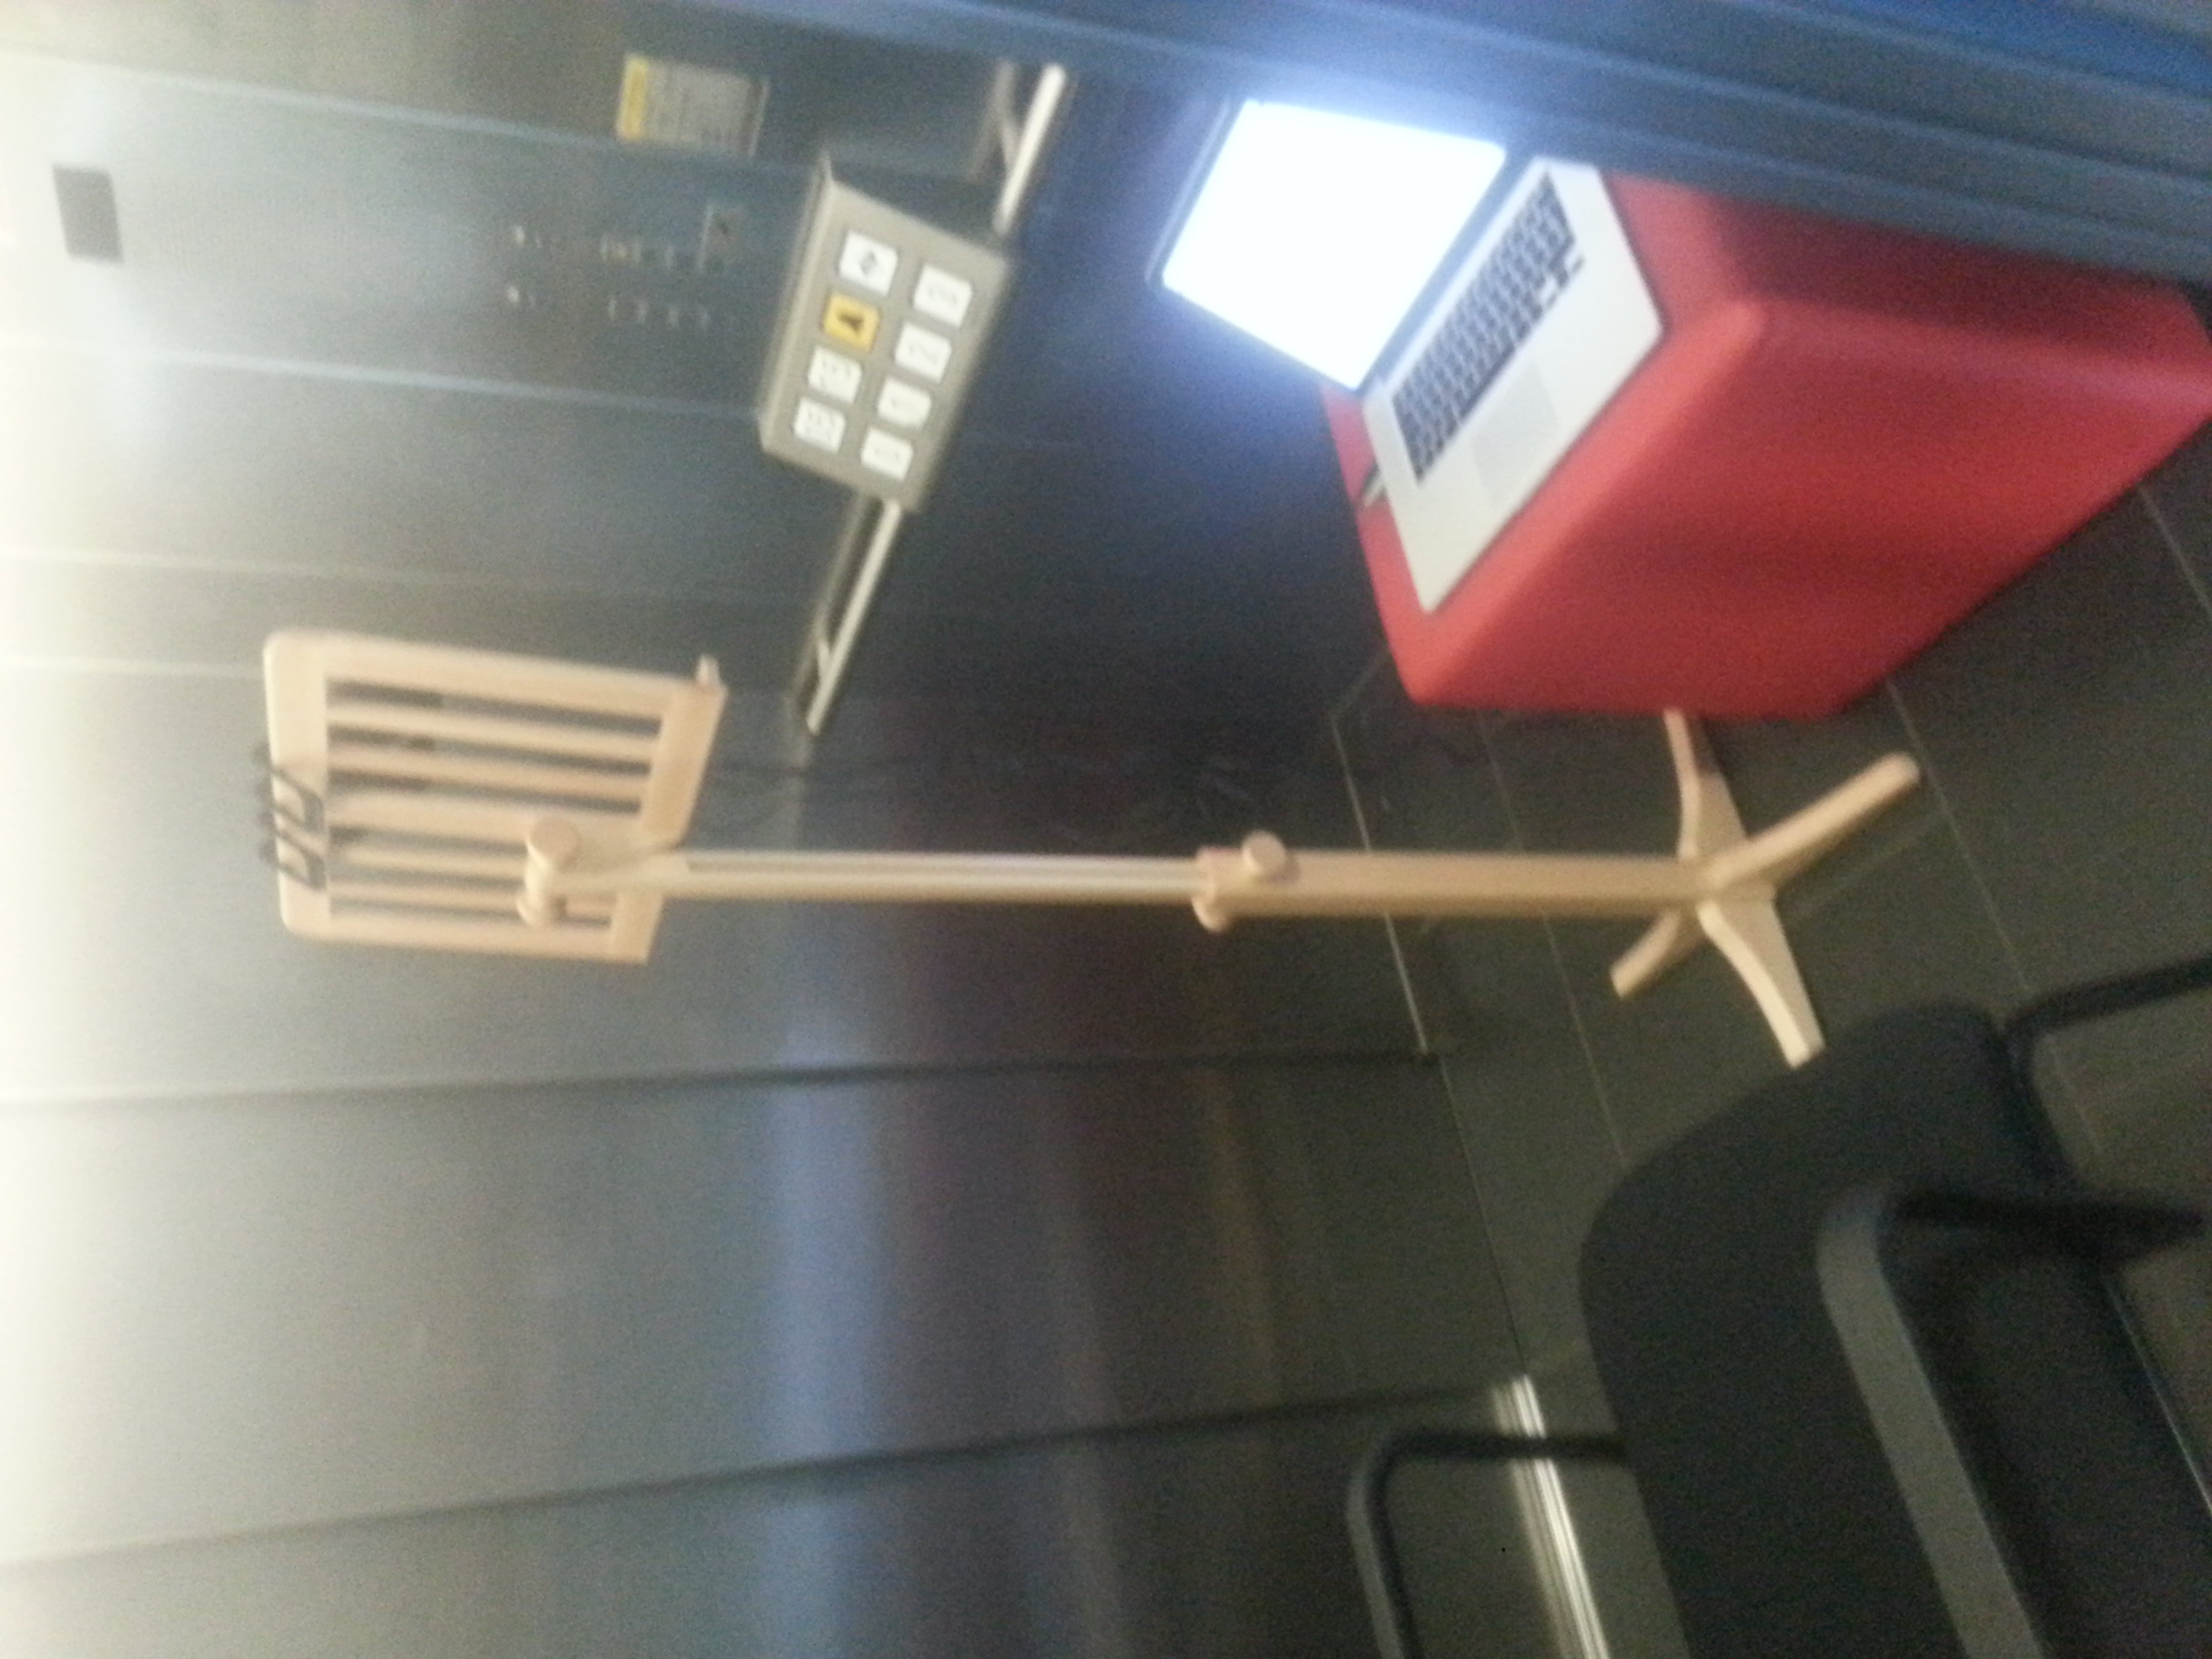
\includegraphics[scale=0.10, angle=-90]{setup_reverberation_rec.jpg}}
%\caption{Recordings setup.}
%\label{fig:recordingsetup}
%\end{figure}

Before working on serial implementation we reviewed several java libraries for serial communication: pi4j, javax.comm, RXTX.
It was decided to stay with RXTX, since pi4j was not stable enough and javax.comm didn't have freely available sources.
Serial implementation follows mainly RXTX examples provided \href{http://rxtx.qbang.org/wiki/index.php/Two_way_communcation_with_the_serial_port}{online} as well as source files of the original project.
For example, floor hex codes and "heartbeat" signal were taken from the original source code.
We also reused several methods from old source files, like the ones that deal with "heartbeat" processing logic.






